% !TEX root = ./document.tex

\documentclass[a4paper, spanish]{article}

\usepackage{mystyle}
\usepackage{myvars}

\begin{document}

  \maketitle

  \begin{itemize}
    \item \textbf{Archivo}: \texttt{weight-loss.csv}
    \item \textbf{Serie}: Frecuencia de búsquedas para la palabra clave \say{Weight loss} a través del buscador \emph{Google} por meses, desde \emph{Enero de 2004} hasta \emph{Diciembre de 2018}. Los valores han sido estandarizados en el rango $[0, 100]$.
  \end{itemize}

  \section{Etapa de identificación}
  \label{sec:1}

    \subsection{Contexto}
    \label{sec:context}

      \paragraph{}
      Tal y como se indica al comienzo de este documento, en este trabajo se va a trabajar con la serie temporal referida a la frecuencia de búsqueda de la palabra clave \say{Weight loss} (a nivel mundial) a través del buscador \emph{Google}. Se ha escogido esta serie para el trabajo por su estructura estacional claramente marcada. Se cree que dicha estructura tiene un alto grado de relación con un índice sobre la preocupación de la población por su peso a lo largo del tiempo.

      \paragraph{}
      Para evitar problemas de privacidad, los datos se proporcionan estandarizados en el rango $[0, 100]$, lo cual elimina la escala de los mismos y únicamente permite estudiar la estructura estocástica de la serie. Esto no es un problema para el análisis que se realizará en este trabajo, dado que precisamente el objetivo del mismo es el de analizar la estructura de una serie serie temporal, siguiendo la metodología de \emph{Box-Jenkins}.

      \paragraph{}
      En cuanto al particionamiento de los datos, estos se proporcionan en agrupaciones mensuales. Dado que se tiene información desde \emph{Enero de 2004} hasta \emph{Diciembre de 2018}, es decir, un total de \emph{15 años}, lo cual suma $15 * 12 = 180$ observaciones en total. Con esta cantidad de observaciones, se cree que se podrá construir un modelo \emph{SARIMA} (\emph{ARIMA} con estacionalidad) de manera adecuada.

      \paragraph{}
      Una vez introducido el contexto de los datos pertenecientes a la serie que se analizará, lo siguiente es empezar a describir la misma a nivel de su estructura estocástica. Tras describir la misma, se procederá a realizar las diferenciaciones pertinentes hasta conseguir que esta sea estacionaria. Una vez se haya conseguido transformar la serie en estacionaria, se tratarán de identificar los parámetros de la parte autoregresiva y de la parte de media móvil, tanto de la dependencia entre observaciones a nivel serial (cada observación con las anteriores), como de la dependencia estacional (cada observación con las anteriores dentro de su periodo estacional). Tras dicha descripción, se propondrán un conjunto de modelos \emph{SARIMA}. En la \autoref{sec:fitting} se prodecerá al ajuste de dichos modelos a los datos. Posteriormente, en la \autoref{sec:comparison} serán descartados aquellos modelos que no puedan validarse por su excesiva falta de ajuste, sobre ajuste, parámetros no significativos, etc. De entre los modelos válidos, se seleccionará aquel cuyo ajuste sea el más próximo a los datos, lo cual se comprobará mediante distintas técnicas. Finalmente, en la \autoref{sec:prediction} se realizará una predicción para el próximo año (\emph{2019}) sobre los valores esperados por el modelo seleccionado.

      \paragraph{}
      La metodología que se ha expuesto en el párrafo anterior se corresponde con la propuesta por \emph{Box-Jenkins} para series temporales basada en ajuste de modelos \emph{ARIMA}. En el documento, se sigue un enfoque en paralelo en lugar de iterativo para la búsqueda del mejor modelo para facilitar la interpretación y la organización del mismo. Esta es la única modificación que se ha llevado a cabo respecto de la metodología original.

    \subsection{Análisis Descriptivo}
    \label{sec:descriptive}


      \paragraph{}
      Tras la descripción de la metodología, se va a comenzar con la descripción de la serie temporal. Para ello, nos vamos a apoyar en los gráficos de la \autoref{img:weightloss}, a partir de los cuales se puede tener una perspectiva completa acerca de la serie. A través de ella se puede ver el gráfico de la serie, el correlograma, el correlograma parcial, el periodograma y el diagrama de dispersión \emph{rango-media}.

      \paragraph{}
      En el gráfico de la serie de la \autoref{img:weightloss} se puede apreciar la evolución temporal de los valores a lo largo de los 15 años, separados en observaciones mensuales. En dicha representación destacan dos características de la serie temporal sobre el resto. Estas son:
        \begin{enumerate*}[label=(\arabic*)]
          \item la marcada estructura estacional de periodo 12 (anual) de la serie, que sigue la misma forma en todas las estacionalidades (años). Esto es un fuerte crecimiento durante el primer mes (Enero), posteriormente se produce un suave decrecimiento hasta el tercer cuarto del año, para producirse un fuerte decrecimiento en torno a los meses de Septiembre - Octubre. Esta estructura estacional es coherente con el fenómeno conocido como \emph{Operación Bikini}, que consiste en la preocupación por estar en buena forma física durante los meses de verano. Esta preocupación comienza en torno a principios de año y se mantiene hasta los meses de verano. Puesto que una vez pasados dichos meses, la forma física deja de estar comprometida, la preocupación por la pérdida de peso de la población también disminuye.
          \item el cambio de nivel que se produce entre el año $2008$ y el año $2009$. Durante este periodo se produce un cambio drástico en el nivel de la serie. Parece que durante el final del año $2008$ no se produjo el fenómeno esperado de un fuerte decrecimiento que sí se produce durante el resto de años. Este cambio en el nivel de la serie pudo deberse a distintos factores, entre los que destaca la crisis económica que comenzó en dicho año. Si se confirma que las razones del aumento del nivel en las búsquedas del término \emph{Weight loss} fueron debidas a la crisis económica, una interpretación para la misma podría ser la siguiente: Con el aumento del riesgo en la estabilidad financiera, la población aumentó también su preocupación en su apariencia física, lo cual se ha mantenido hasta la actualidad. Otros factores podrían ser el acercamiento de la tecnología y redes sociales al gran público, que hasta entonces se habían mantenido alejadas del mismo.
        \end{enumerate*}

      \begin{figure}[htb!]
        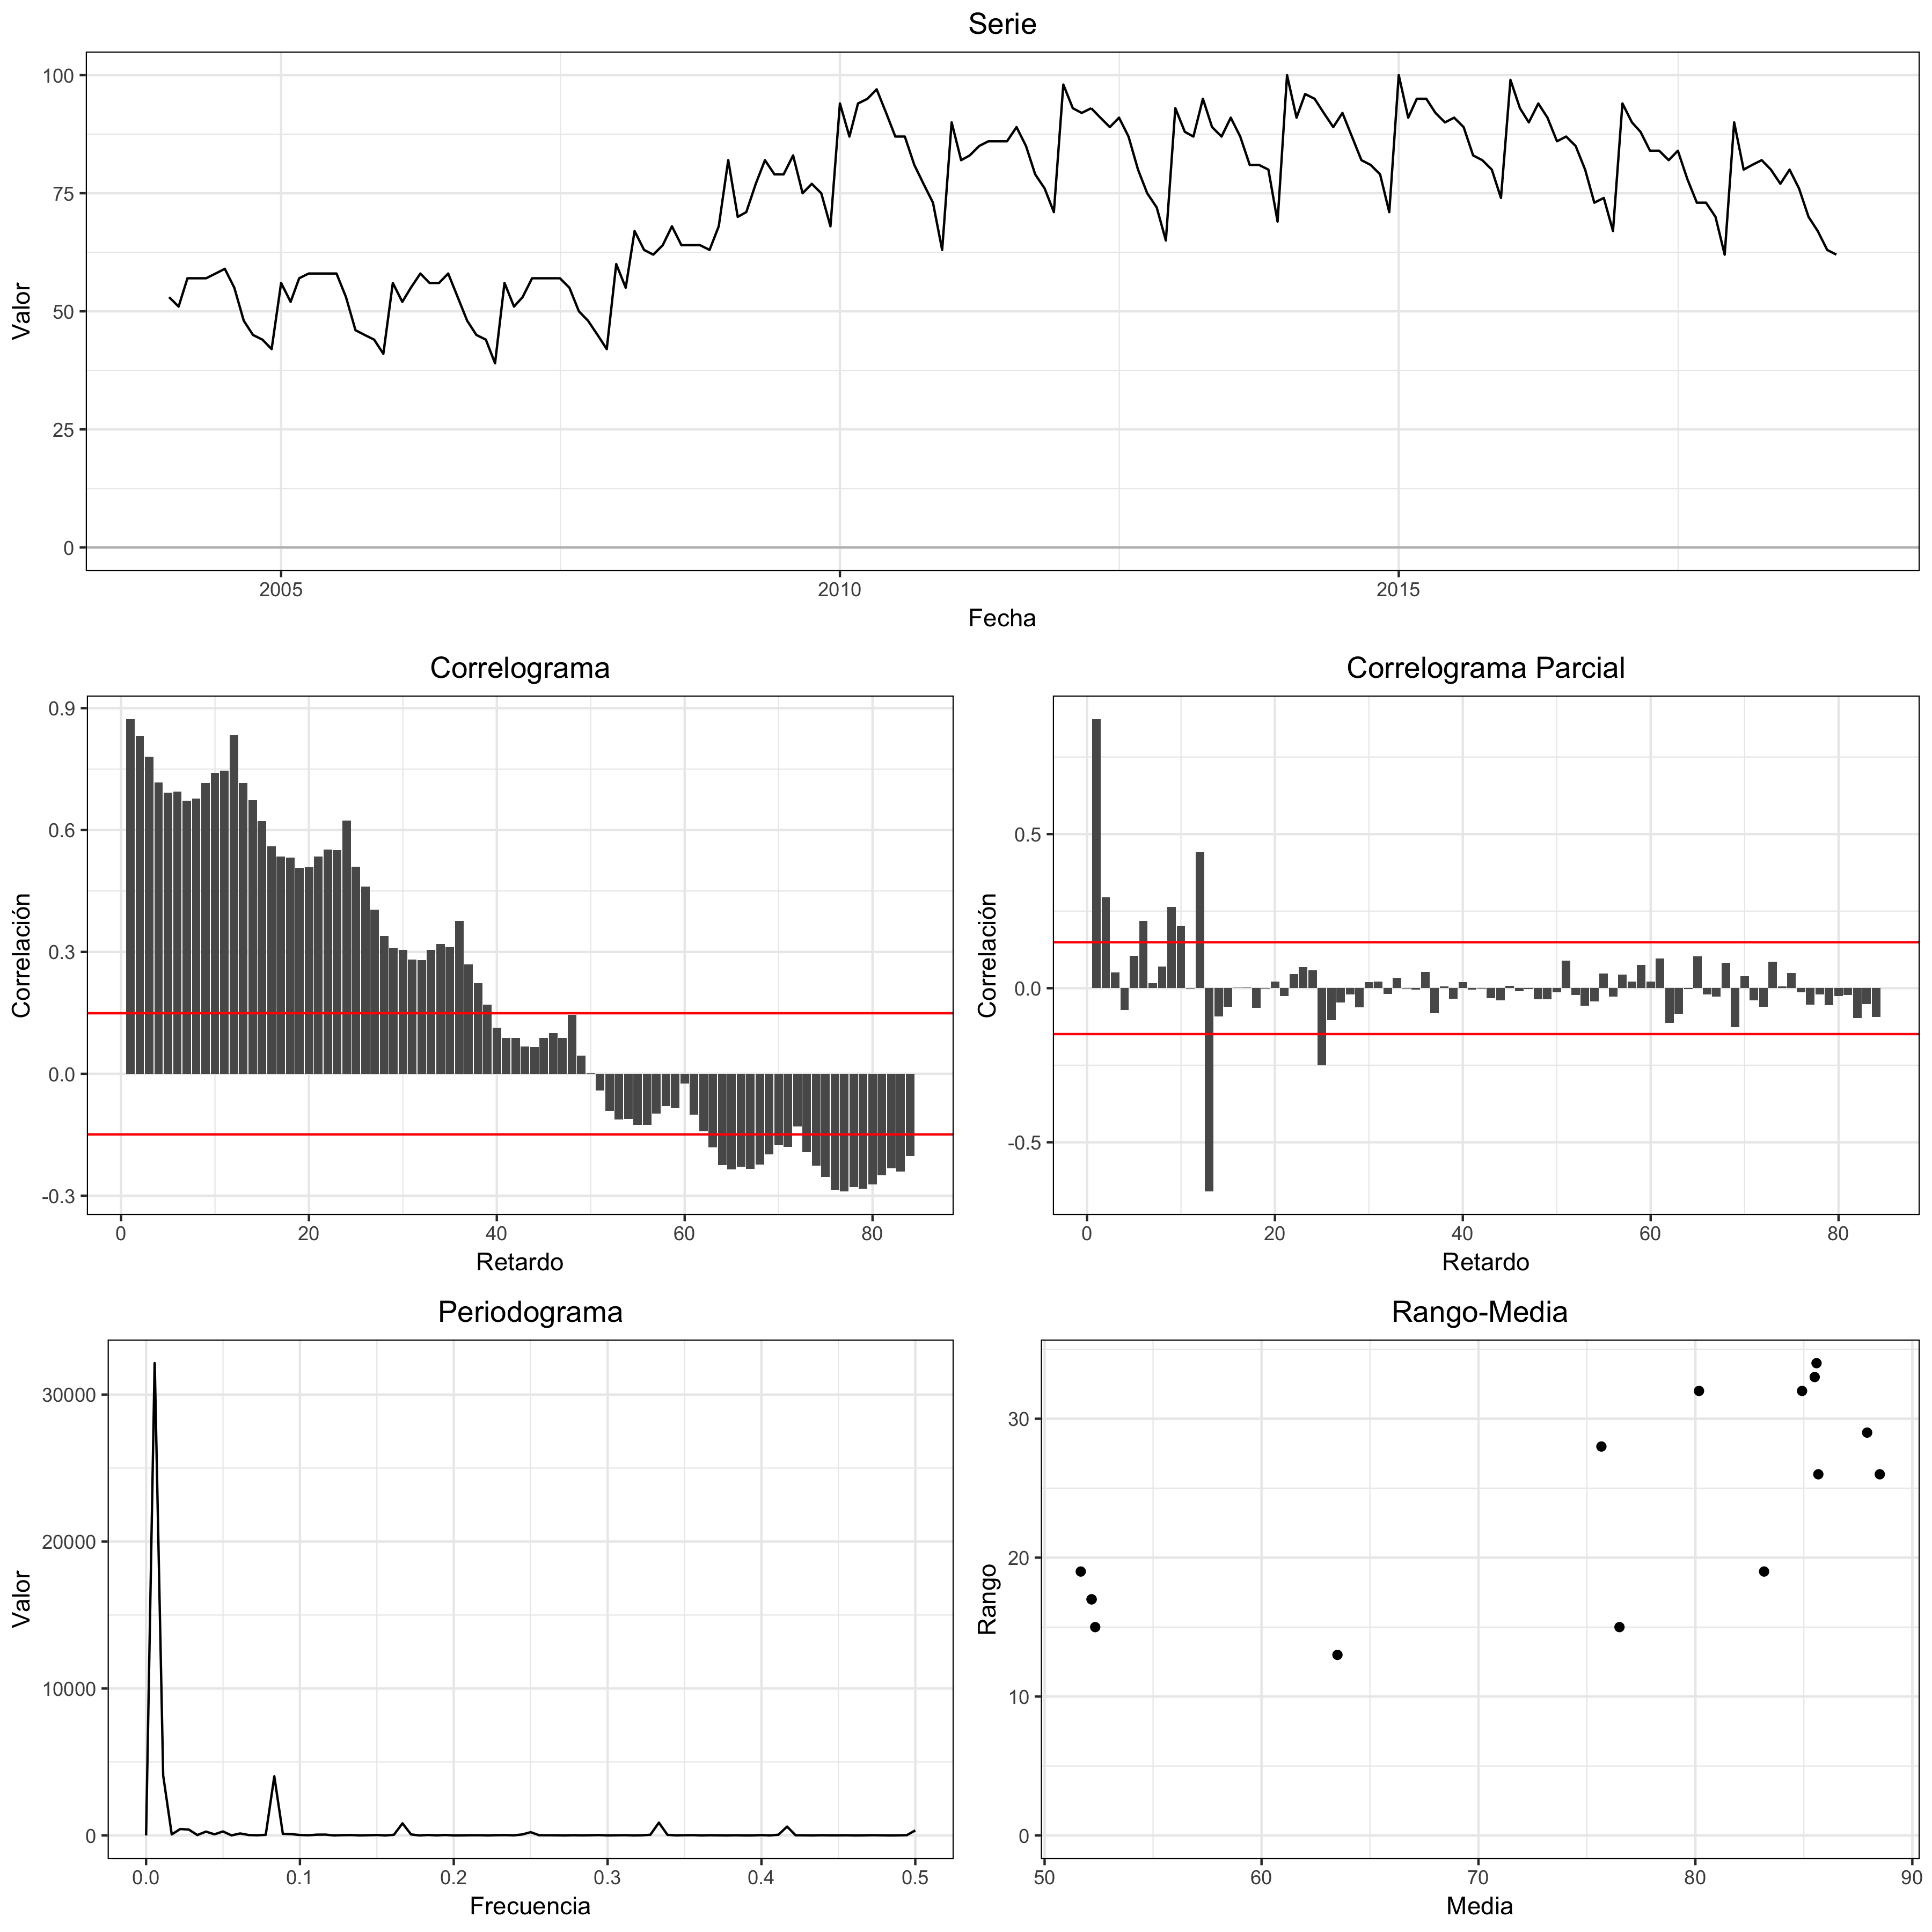
\includegraphics[width=\textwidth,height=\textheight,keepaspectratio]{weightloss}
        \caption{Gráfico de la serie, Correlograma, Correlograma Parcial, Periodograma y diagrama de dispersión \emph{rango-media} para la serie \texttt{weightloss}.}
        \label{img:weightloss}
      \end{figure}

      \paragraph{}
      En cuanto al correlograma de la serie que se muestra en la \autoref{img:weightloss}, se puede apreciar la componente estacional de periodo 12 en la estructura de correlaciones. Destacan sobre el resto los retardos de la forma $i \text{ mod } 12 = 0$, estos son los retardos $12, 24, 36,...$. Estos se relacionan entre si presentando un decrecimiento lineal, por lo que son indicativo de que la serie no es estacionaria. Por lo tanto, tendremos que llevar a cabo al menos una diferenciación estacional para conseguir estacionarizar la serie. También llama la atención la gran cantidad de correlaciones con valores significativos, por lo que la tendencia podría estar ocultando algún otro comportamiento no visible a simple vista. Por lo tanto, la realización de una diferenciación regular también podría ser una buena estrategia para tratar de comprender en mayor medida la estructura de correlaciones de la serie. Tal y como se verá en el siguiente párrafo, estas interpretaciones se ven reflejadas en el correlograma parcial.

      \paragraph{}
      En el correlograma parcial de la serie de la \autoref{img:weightloss} se representan las correlaciones entre observaciones de la serie, tratando de eliminar de estas la relación procedente de otros retardos. Es decir, el correlograma parcial trata de representar de manera aislada la correlación entre una observación y la del $k$-ésimo retardo posterior, eliminando la influencia del resto. En este caso destacan sobre el resto los retardos $1$, $12$ y $13$. Se cree que el retardo $1$ destaca sobre el resto debido a la tendencia de la serie mientras que el retardo $12$ se debe a la estacionalidad de la misma. También se piensa que el retardo $13$ es un reflejo del $1$, en la estacionalidad anterior, de ahí la razón de que destaque de tal manera.

      \paragraph{}
      En cuanto al periodograma de la serie que se muestra en la \autoref{img:weightloss}, se puede apreciar que el primer armónico recoge gran parte de la variabilidad de la serie, lo cual de nuevo vuelve a indicar que la tendencia de la misma puede estar ocultando información sobre la estructura estocástica de la serie. Por lo tanto, se cree que una diferenciación permitiría visualizar en mayor medida el comportamiento de la misma. También destacan (aunque de una manera mucho menos pronunciada) los armónicos de la forma $i + 1 / 12$ con $i \in {1, 2, ..., 6}$, esto es $1/12, 2/12, ..., 6/12$, lo cual es otro argumento de peso en favor de la componente estacional de periodo $12$ (anual) de la serie.

      \paragraph{}
      En cuanto al diagrama de dispersión \emph{rango-media} de la \autoref{img:weightloss}, parece que exista una leve relación entre el nivel de la serie y la dispersión del mismo. Este fenómeno podría requerir de alguna transfomación de estabilización de varianza, como las de la forma \emph{Box-Cox}. La razón de ello es que los modelos que se ajustarán a la serie temporal requieren de estacionaridad en la serie (entre otros requisitos, la varianza debe ser constante a lo largo de la serie). Sin embargo, tal y como se verá posteriormente, las diferenciaciones eliminarán la relación entre nivel y dispersión, por lo que es algo de lo que no nos preocuparemos en gran medida.


    \subsection{Diferenciaciones}
    \label{sec:differences}

      \paragraph{}
      [TODO]

      \subsubsection{Diferenciación regular}

        \paragraph{}
        [TODO]

        \begin{figure}[htb!]
          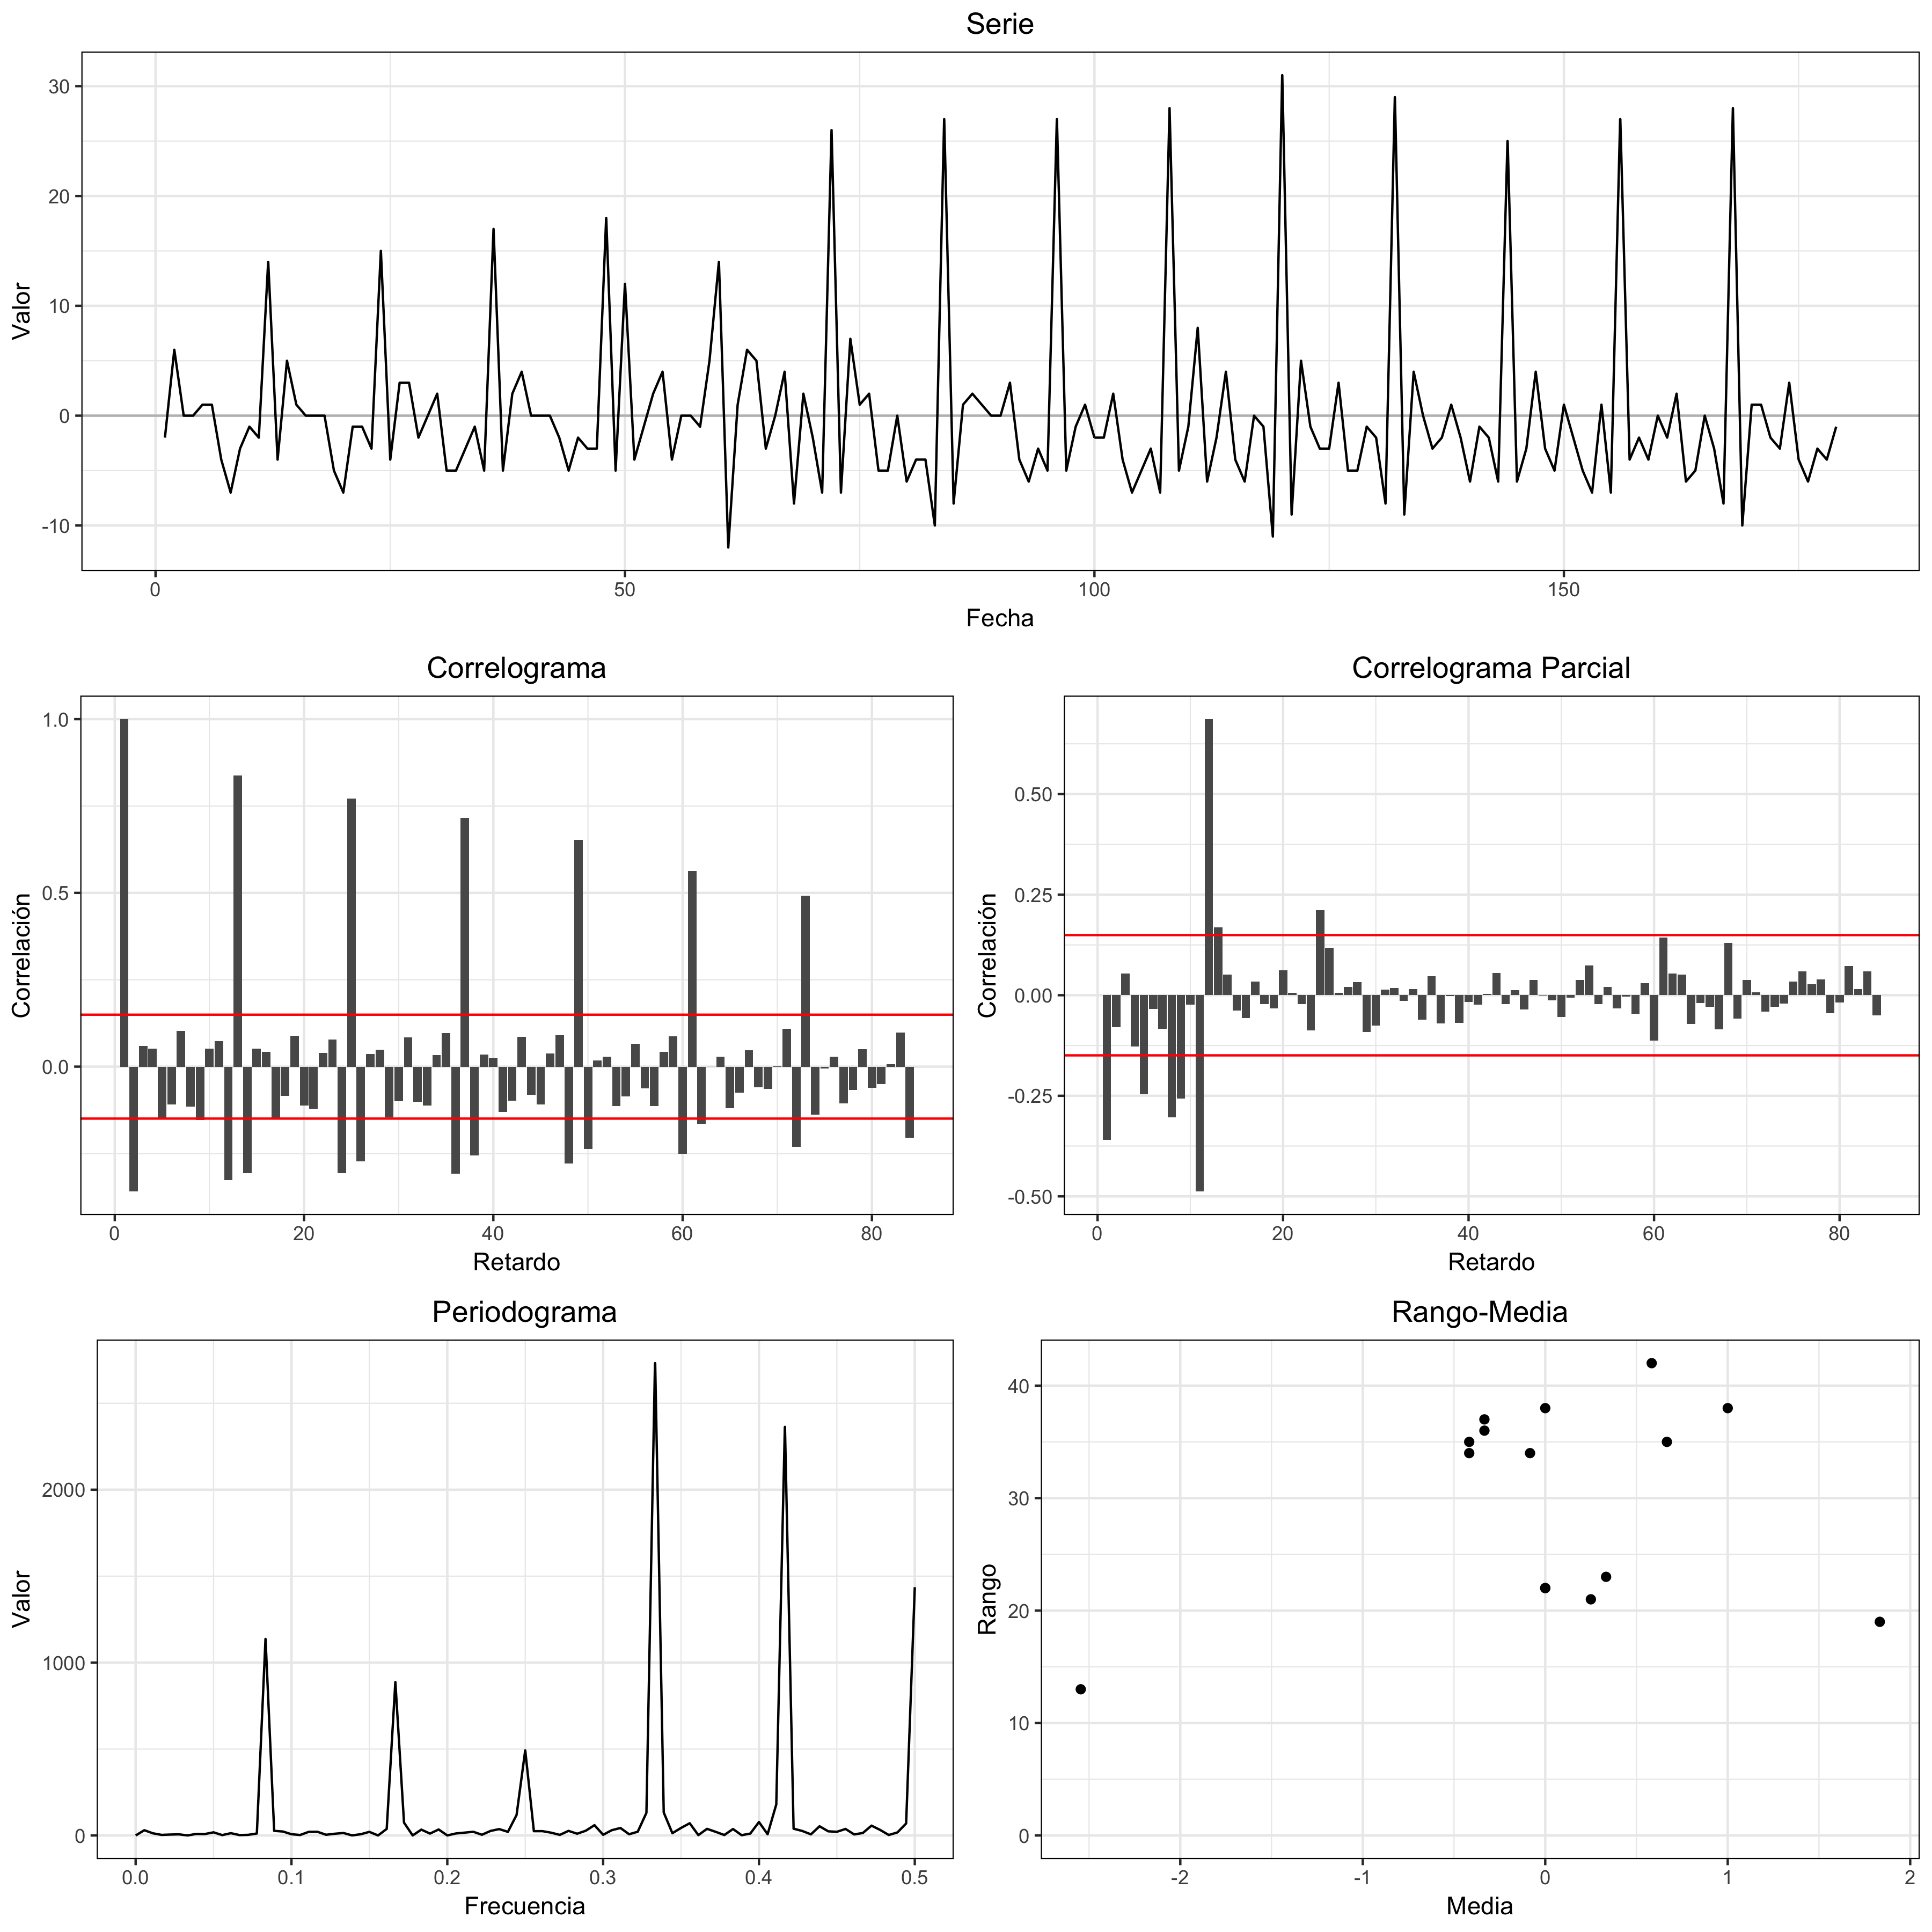
\includegraphics[width=\textwidth,height=\textheight,keepaspectratio]{weightloss-diff-1}
          \caption{Gráfico de la serie, Correlograma, Correlograma Parcial, Periodograma y diagrama de dispersión \emph{rango-media} para la serie \texttt{weightloss} tras la realización de una diferenciación regular.}
          \label{img:weightloss_diff_1}
        \end{figure}

      \subsubsection{Diferenciación estacional}


        \paragraph{}
        [TODO]

        \begin{figure}[htb!]
          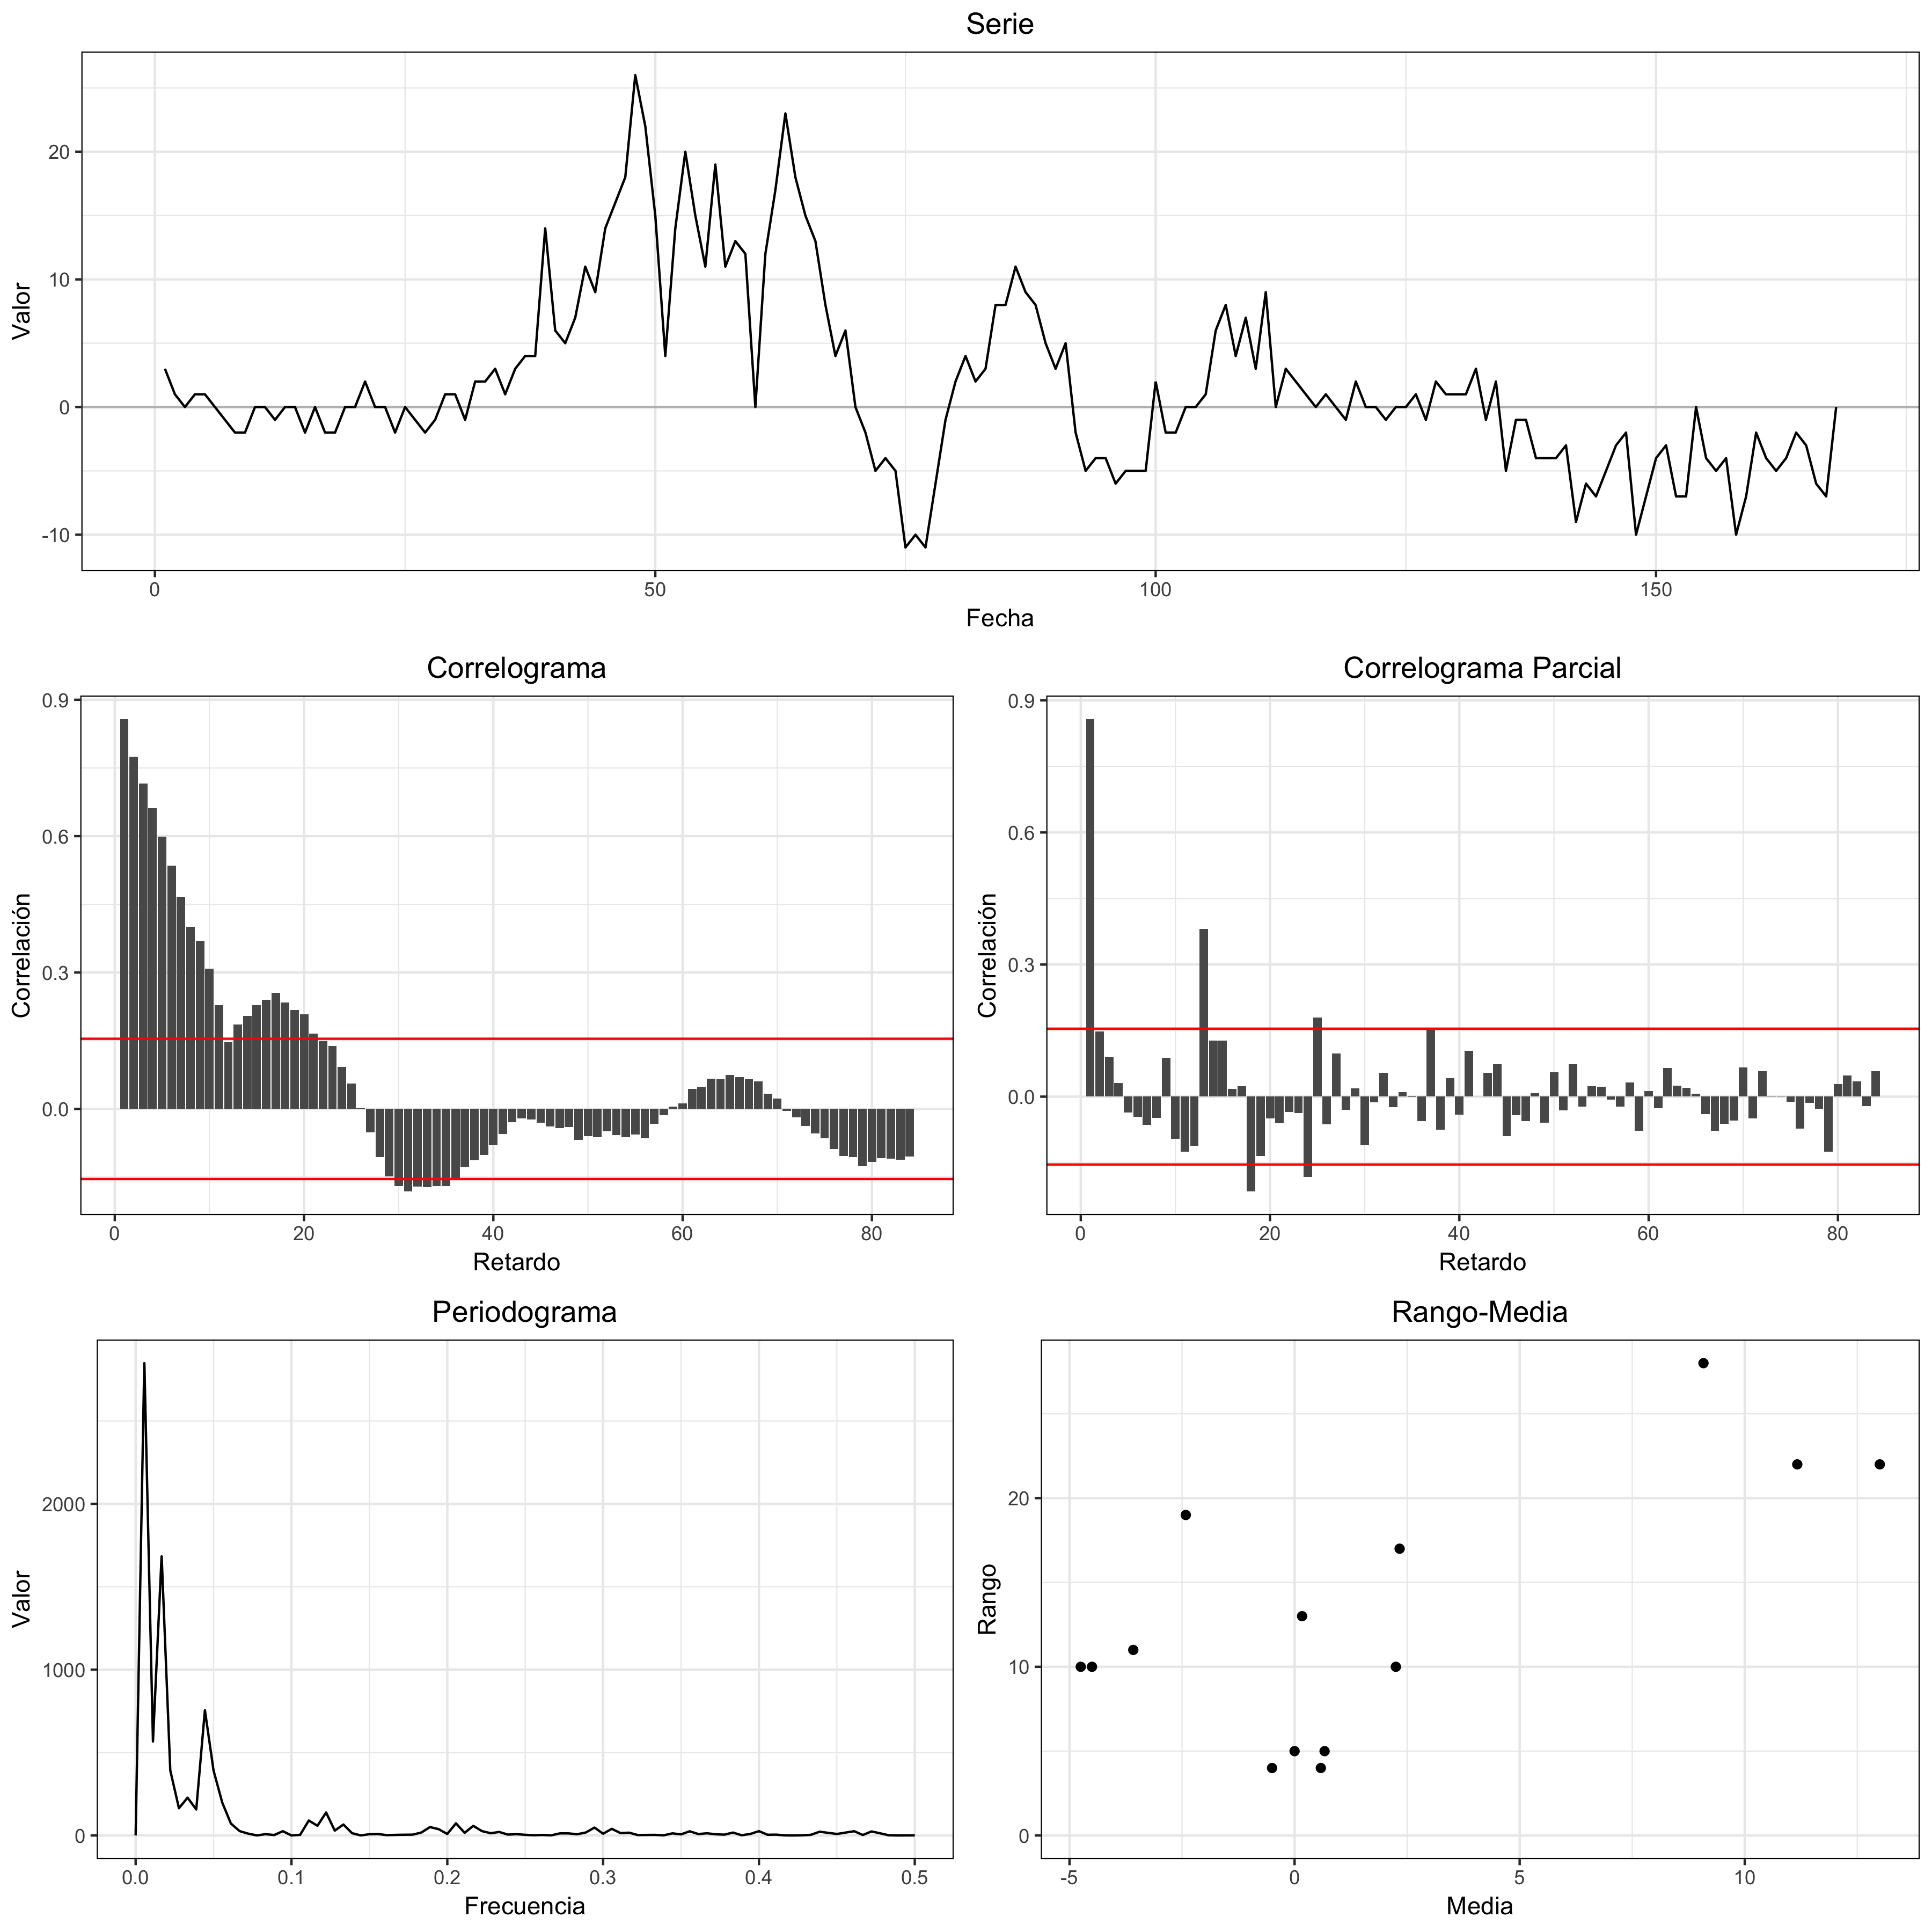
\includegraphics[width=\textwidth,height=\textheight,keepaspectratio]{weightloss-diff-12}
          \caption{Gráfico de la serie, Correlograma, Correlograma Parcial, Periodograma y diagrama de dispersión \emph{rango-media} para la serie \texttt{weightloss} tras la realización de una diferenciación estacional (12 retardos).}
          \label{img:weightloss_diff_12}
        \end{figure}

      \subsubsection{Diferenciación regular y estacional}

        \paragraph{}
        [TODO]

        \begin{figure}[htb!]
          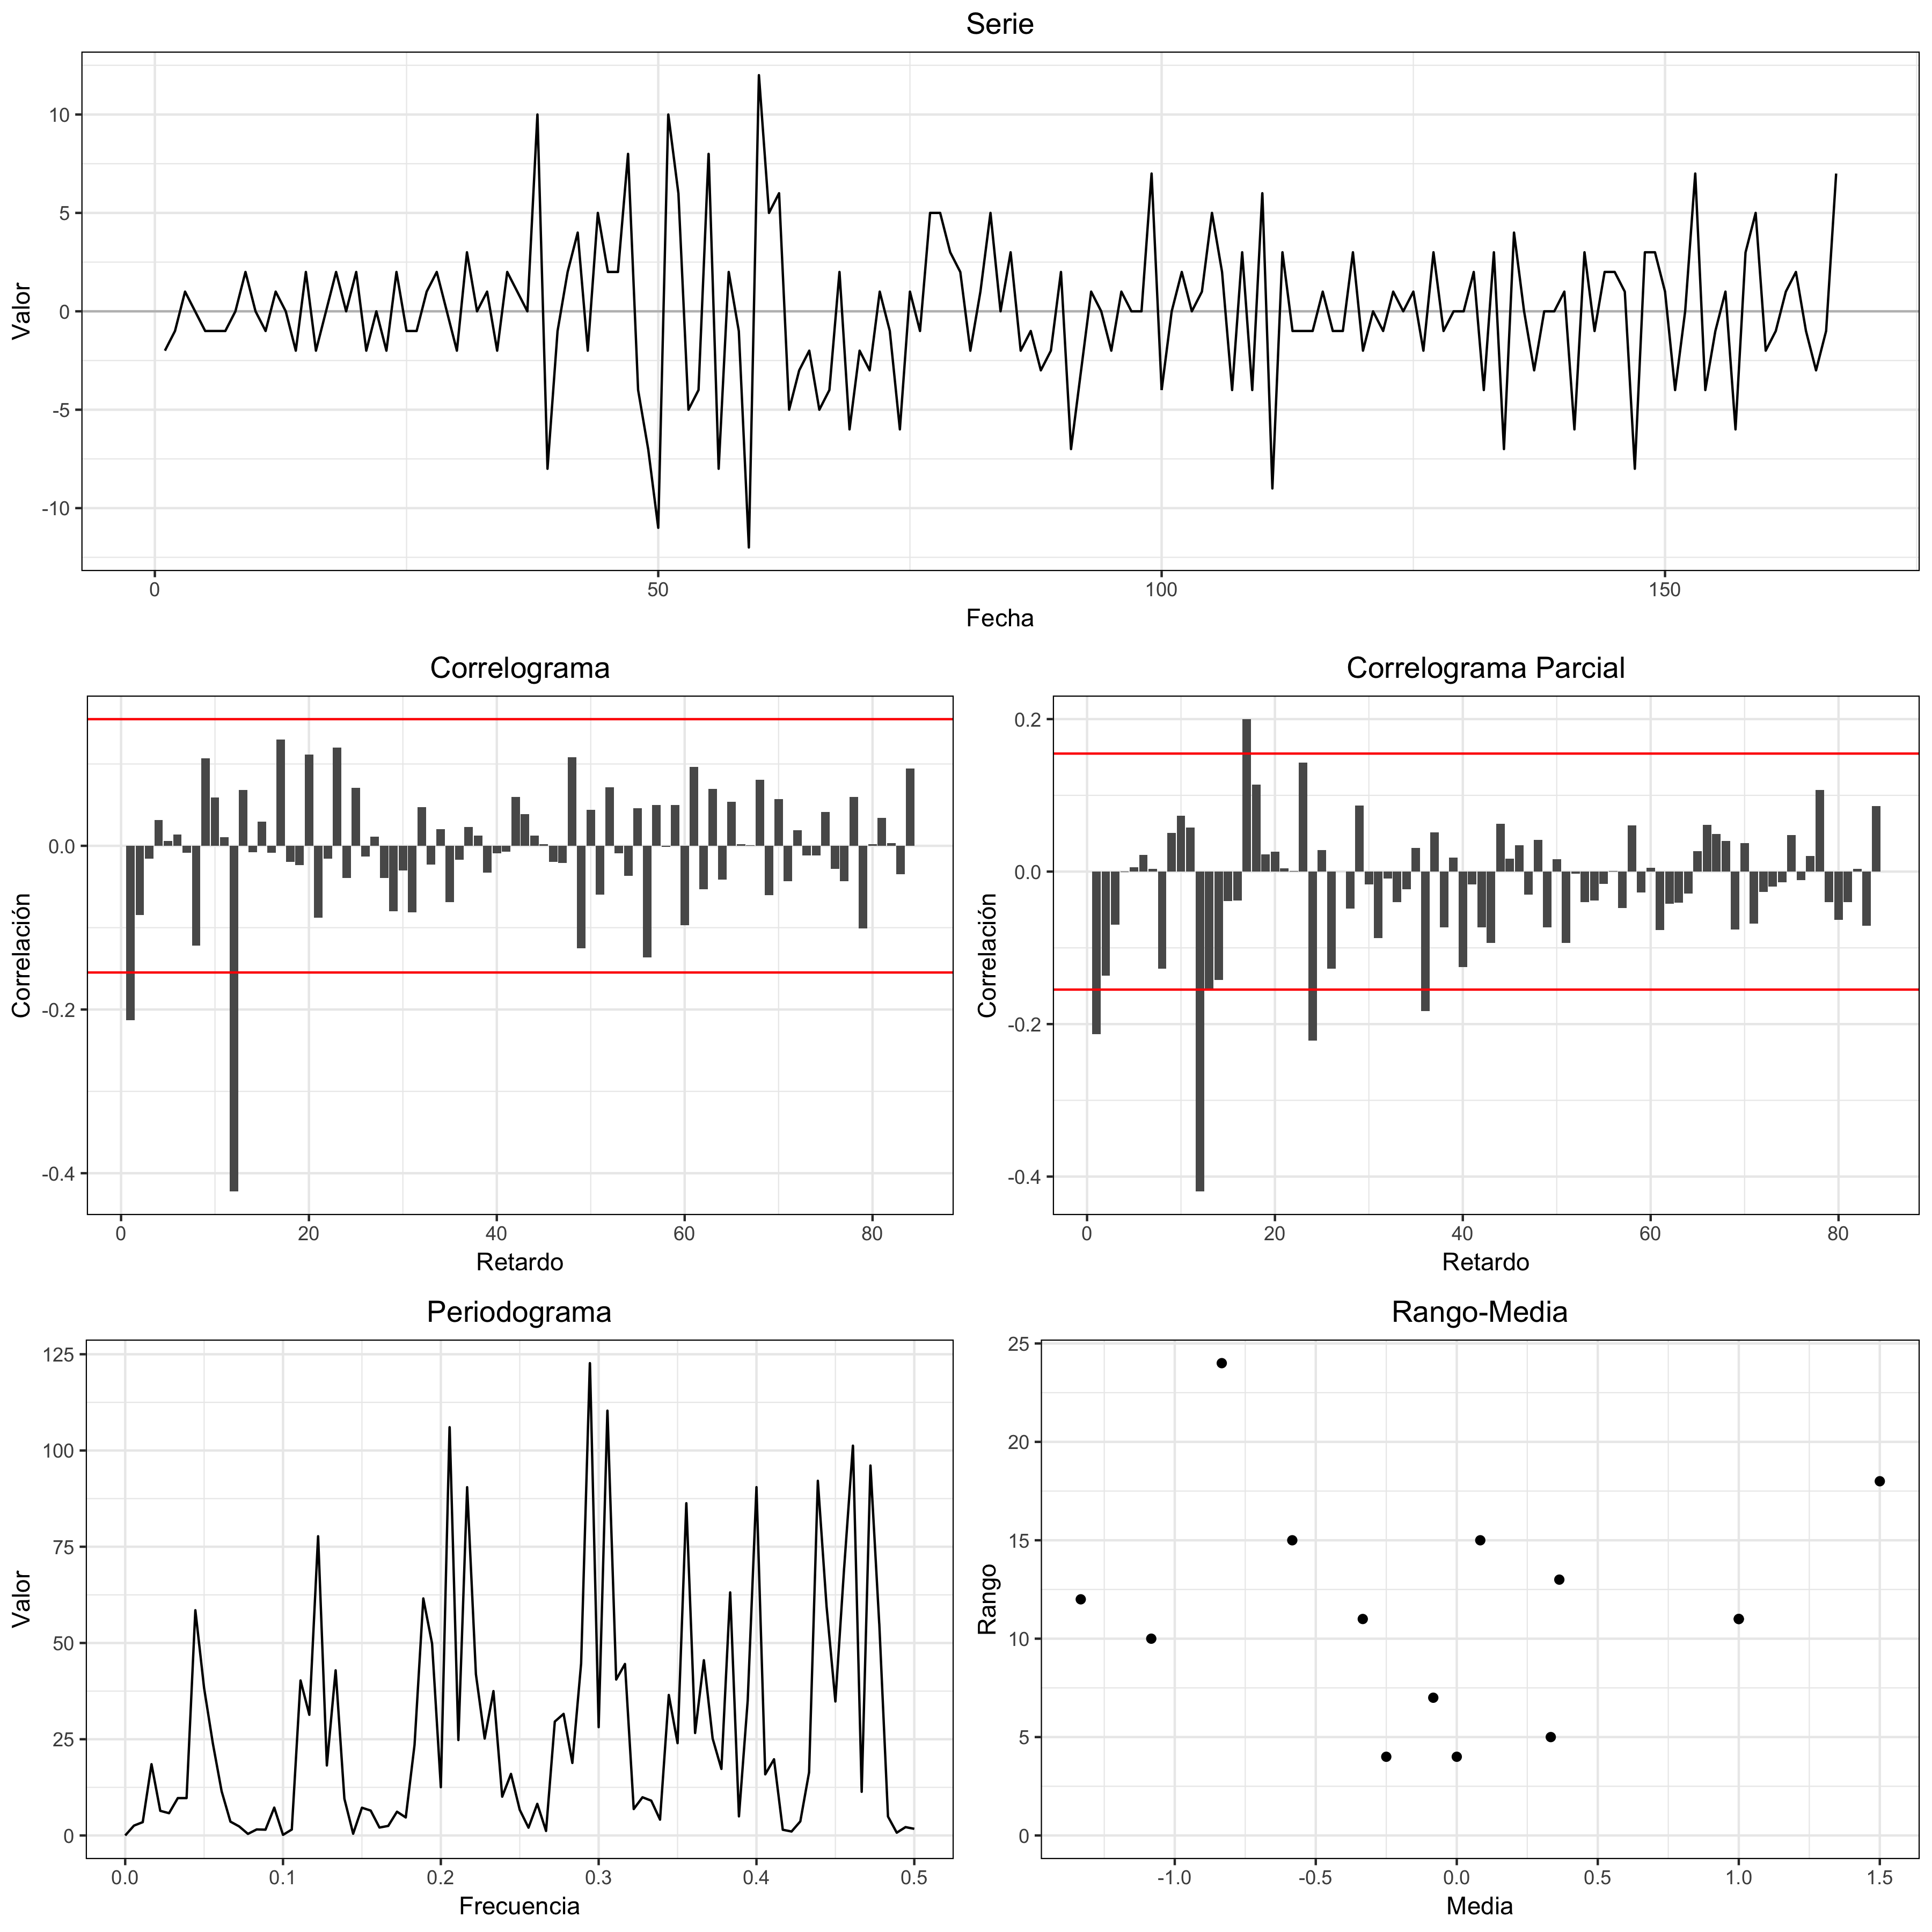
\includegraphics[width=\textwidth,height=\textheight,keepaspectratio]{weightloss-diff-1-12}
          \caption{Gráfico de la serie, Correlograma, Correlograma Parcial, Periodograma y diagrama de dispersión \emph{rango-media} para la serie \texttt{weightloss} tras la realización de una diferenciación regular y otra diferención estacional (12 retardos).}
          \label{img:weightloss_diff_1_12}
        \end{figure}

    \paragraph{}
    [TODO]

    \subsection{Modelos propuestos}
    \label{sec:proposed_models}

      \paragraph{}
      [TODO]

  \section{Etapa de estimación y validación}
  \label{sec:fitting}

    \paragraph{}
    [TODO]

  \section{Comparación de modelos}
  \label{sec:comparison}

    \paragraph{}
    [TODO]

  \section{Predicción}
  \label{sec:prediction}

    \paragraph{}
    [TODO]

  \appendix
  \section{Código Fuente}
  \label{sec:code}

    \paragraph{}
    [TODO]


    \begin{listing}[H]
        \centering
        \inputminted{R}{./res/code/weight-loss.r}
        \caption{[TODO]}
        \label{}
      \end{listing}
\end{document}
